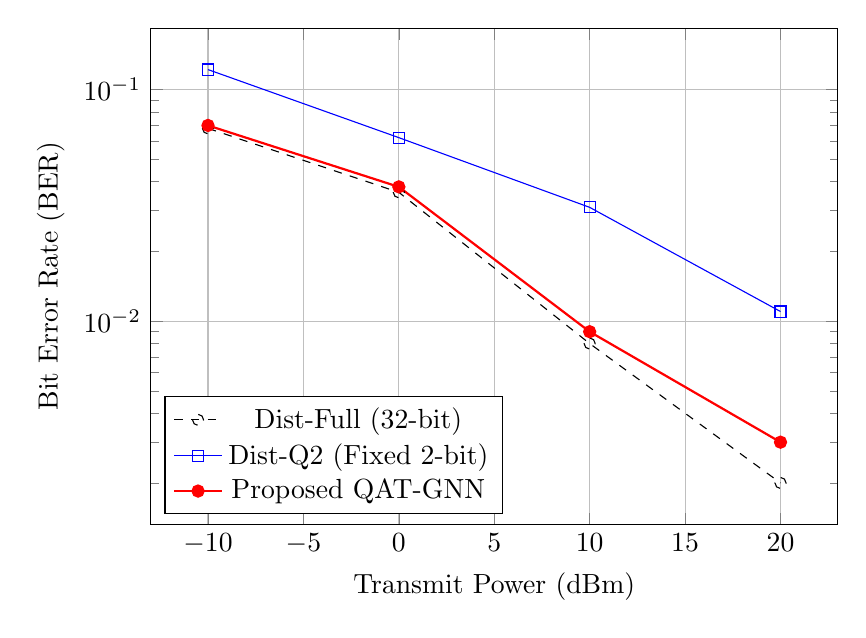
\begin{tikzpicture}
\begin{semilogyaxis}[
    xlabel={Transmit Power (dBm)},
    ylabel={Bit Error Rate (BER)},
    grid=major,
    legend style={at={(0.02,0.02)},anchor=south west},
    width=0.85\linewidth,
    height=0.65\linewidth
]
\addplot[color=black, mark=o, dashed] coordinates {(-10, 0.068) (0, 0.036) (10, 0.008) (20, 0.002)}; \addlegendentry{Dist-Full (32-bit)}
\addplot[color=blue, mark=square] coordinates {(-10, 0.122) (0, 0.062) (10, 0.031) (20, 0.011)}; \addlegendentry{Dist-Q2 (Fixed 2-bit)}
\addplot[color=red, mark=*, thick] coordinates {(-10, 0.070) (0, 0.038) (10, 0.009) (20, 0.003)}; \addlegendentry{Proposed QAT-GNN}
\end{semilogyaxis}
\end{tikzpicture}